\pdfminorversion=4
\documentclass[compress,10pt]{beamer}
%For no animations, add handout to [] options
%For no figures or top banner, add draft to [] options
%apsectratio=169 (16:9) or 54 (5:4) or 43 (4:3) or 32 (3:2)

%Load the myriad packages
\usepackage{color}
\usepackage{amssymb,amsmath}
\usepackage{textcomp}
\usepackage{graphicx}
\usepackage{tikz}
%\usepackage[numbers, super]{natbib}
\usepackage{grffile} %spaces in file names
\usepackage{parskip}
%\usepackage[T1]{fontenc} %for sc and bf
%\usepackage{times}
\usepackage{wasysym}
\usepackage{bigstrut}
\usepackage{epstopdf}
%\usepackage{enumitem}
%\setlist{nolistsep} % or \setlist{noitemsep} to leave space around whole list
% Load some optional sub-parts of PGF
%\usetikzlibrary{decorations.pathmorphing}
%\usetikzlibrary{positioning}
%\usetikzlibrary{calc}
%\usetikzlibrary{shapes.geometric}
%\usepackage{pgfplots}
%\usepackage{rotating}
%\usepackage[no-math]{fontspec}
%\usepackage{xltxtra}
%\usepackage{xunicode}
%\defaultfontfeatures{Mapping=tex-text}
%%\setsansfont[Mapping=tex-text]{Optima}
%\setsansfont[Mapping=tex-text]{Helvetica Neue}
% Optional for code samples
%
%singular
\newcommand{\fref}[1]{Fig.~\ref{fig:#1}}
\newcommand{\Fref}[1]{Figure~\ref{fig:#1}}
\newcommand{\eref}[1]{Eq.~(\ref{eq:#1})}
\newcommand{\Eref}[1]{Equation~(\ref{eq:#1})}
\newcommand{\tref}[1]{Table~\ref{tab:#1}}
%plural
\newcommand{\frefs}[2]{Figs.~\ref{fig:#1} and \ref{fig:#2}}
\newcommand{\Frefs}[2]{Figures~\ref{fig:#1} and \ref{fig:#2}}
\newcommand{\erefs}[2]{Eqs.~(\ref{eq:#1}) and (\ref{eq:#2})}
\newcommand{\Erefs}[2]{Equations~(\ref{eq:#1}) and (\ref{eq:#2})}
\newcommand{\trefs}[2]{Tables~\ref{tab:#1} and \ref{tab:#2}}
%range
\newcommand{\frefss}[2]{Figs.~\ref{fig:#1} - \ref{fig:#2}}
\newcommand{\Frefss}[2]{Figures~\ref{fig:#1} - \ref{fig:#2}}
\newcommand{\erefss}[2]{Eqs.~(\ref{eq:#1}) - (\ref{eq:#2})}
\newcommand{\Erefss}[2]{Equations~(\ref{eq:#1}) - (\ref{eq:#2})}
\newcommand{\trefss}[2]{Tables~\ref{tab:#1} - \ref{tab:#2}}
%misc.
\newcommand{\nn}[1]{\ensuremath{^{#1}}} %[1] is # of commands
\newcommand{\keff}{\ensuremath{{k_\mathrm{eff}}}}
\newcommand{\kinf}{\ensuremath{{k_\infty}}}
\newcommand{\alphaT}{\ensuremath{{\alpha_{_T}}}}
\newcommand{\SN}{\ensuremath{{\text{S}_\text{N}}}}
\newcommand{\order}[1]{\ensuremath{\mathcal{O}\left(#1\right)}}
%Note: tarticle has ``several'' changes from article
%in this vein.
% some simplifying commands
\newcommand{\eg}{{\it e.g.}}
\newcommand{\ie}{{\it i.e.}}
\newcommand{\etal}{{\it et al.}}
\newcommand{\acite}[1]{{\bf(Add Citation: #1)}}
\newcommand{\E}{\mathcal{E}}
% derivative - d
\newcommand{\ud}{\,\mathrm{d}}
% bold unit vector n-hat
\newcommand{\nhat}{\hat{\bf n}}
\newcommand{\tensor}[1]{\mathcal{#1}}
\renewcommand{\vec}[1]{\mathbf{#1}}
\newcommand{\om}{\boldsymbol{\Omega}}
%

%Don't number backup slides
\newcommand{\backupbegin}{
    \newcounter{finalframe}
    \setcounter{finalframe}{\value{framenumber}}
}
\newcommand{\backupend}{
    \setcounter{framenumber}{\value{finalframe}}
}

%Colors!
\definecolor{maroon}{rgb}{0.5,0,0}
\definecolor{darkgreen}{rgb}{0,0.5,0}

%Get rid of navigation icons
\setbeamertemplate{navigation symbols}{}
\useoutertheme{infolines}

\setbeamercovered{transparent}
\usepackage{lipsum}

%Aggie-themed
\pgfdeclareimage[height=0.1in]{TAMUlogo}{images/tamu_engineering.png}
\pgfdeclareimage[height=0.15in]{DOElogo}{images/DOE_logo.png}
\logo{\raisebox{-8pt}{\pgfuseimage{TAMUlogo} \hspace{1pt} \pgfuseimage{DOElogo}}}
\titlegraphic{
\includegraphics[height=0.15\textheight]{images/seal.png}}

%%%%%%%%%%%%%%%%%%%%%%%%%%%%%%%%%%%%%%%%%%%%%%%%%%%%%%%%%%%%%%%
% Optional packages, used to show off certain tricks

\newlength \figwidth
\setlength \figwidth {0.5\textwidth}

\setlength{\leftmargin}{-2cm}
\setlength{\rightmargin}{-2cm}

%%%%%%%%%%%%%%%%%%%%%%%%%%%%%%%%%%%%%%%%%%%%%%%%%%%%%%%%%%%%%%%

\mode<presentation>
{
    \usepackage[english]{babel}
    \usetheme{Frankfurt}

    %Make it Aggie Maroon
    \usecolortheme[RGB={80,0,0}]{structure}

    % This will typeset only the frames (or slides) that have the given label ("current" in this case).
    %  \includeonlyframes{current}
}

\title[Polytope DGFEM Transport]{Higher-Order DGFEM Transport Calculations on Polytope Meshes for Massively-Parallel Architectures}

\author[Hackemack]{{\Large Michael W. Hackemack} \vspace{0.35cm} \\ Chair: {\small Jean C. Ragusa} \\ Committee Members: {\small Marvin L. Adams, Jim E. Morel, Nancy M. Amato } \\ External Advisor: {\small Troy Becker}}

%TAMU
\institute[Texas A\&M University]{\scriptsize Department of Nuclear Engineering\\
Texas A\&M University \\
College Station, TX, USA 77843\\[1ex]
\href{mailto:mike\_hack@tamu.edu}{mike\_hack@tamu.edu}}

\date[November 24, 2015]

% You can override the default acknowledgment, and address if you want
%\acknowledgement{*Submitted in partial fulfillment of the requirements of NUEN 610 \\
%(Nuclear Reactor Design)}
%\address{Nuclear Engineering Department \\
%            Texas A\&M University \\
%            College Station, TX 77843-3133}}

% If you don't want the menu section outline above the title, do this:
%\setbeamertemplate{headline}{}

\renewcommand{\ss}{ss}
\vfuzz=2pt

%%%%%%%%%%%%%%%%%%%%%%%%%%%%%%%%%%%%%%%%%%%%%%%%%%%%%%%%%%%%%%%%%%%%%%%%%%%%%%%%%%%%%%%%%%%%%
\begin{document}

%%%%%%%%%%%%%%%%%%%%%%%%%%%%%%%%%%%%%%%%%%%%%%%%%%%%%%%%%%%%%%%%%%%%%%%%%%%%%%%%%%%%%%%%%%%%%
%  All this typeout stuff simply gets printed to the screen as the document
% is compiled.  It helps get stuff working
\typeout{***********************************************************************************}
\typeout{titlepage}

\begin{frame}[label=title,plain]
    \titlepage
\end{frame}

%%%%%%%%%%%%%%%%%%%%%%%%%%%%%%%%%%%%%%%%%%%%%%%%%%%%%%%%%%%%%%%%%%%%%%%%%%%%%%%%%%%%%%%%%%%%%%
\typeout{***********************************************************************************}
\typeout{TOC}

\begin{frame}[shrink,label=toc,plain]%[plain]
    \frametitle{Outline}
    \vspace{1.1mm}
    \tableofcontents
\end{frame}

%%%%%%%%%%%%%%%%%%%%%%%%%%%%%%%%%%%%%%%%%%%%%%%%%%%%%%%%%%%%%%%%%%%%%%%%%%%%%%%%%%%%%%%%%%%%%%
%
\section{Overview}
\subsection{The DGFEM $S_N$ Transport Equation}

%%%%%%%%%%%%%%%%%%%%%%%%%%%%%%%%%%%%%%%%%%%%%%%%%%%%%%%%%%%%%%%%%%%%%%%%%%%%%%%%%%%%%%%%%%%%%
\typeout{***********************************************************************************}
\typeout{The DGFEM $S_N$ Transport Equation}
\begin{frame}[t]\frametitle{The Continuous-Energy Transport Equation}
\begin{block}{Transport Equation}{\footnotesize
\begin{equation*}
\left[ { \bf \Omega} \cdot {\bf \nabla}  + \sigma_t ({\bf r}, E) \right] \psi ({\bf r}, E, {\bf \Omega}) = \int_{4 \pi} \int_{0}^{\infty}  \, \sigma_s ({\bf r}, E' , E, {\bf \Omega}' , {\bf \Omega}) \psi ({\bf r}, E', {\bf \Omega}') d E'  d \Omega'+ Q ({\bf r}, E, {\bf \Omega})
\end{equation*}
}\end{block}
\begin{block}{Boundary Conditions}{\footnotesize
\begin{equation*}
\psi ({\bf r}, E, {\bf \Omega}) = \psi^{inc} ({\bf r}, E, {\bf \Omega}) +  \int_{4 \pi} \int_{0}^{\infty} \beta ({\bf r}, E' , E, {\bf \Omega}' , {\bf \Omega}) \psi ({\bf r}, E', {\bf \Omega}') d E'  d \Omega'
\end{equation*}
}\end{block}
\begin{block}{Term Definitions} {\footnotesize
${\bf r}$ -  neutron position \\
$E$ -  neutron energy \\
${\bf \Omega}$ - neutron solid angle \\
$\psi  ({\bf r}, E, {\bf \Omega})$ - angular flux  \\
$Q  ({\bf r}, E, {\bf \Omega})$ - distributed neutron source \\
$\sigma_t ({\bf r}, E)$ - total macroscopic cross section \\
$\sigma_s ({\bf r}, E' , E, {\bf \Omega}' , {\bf \Omega})$ - total macroscopic scattering cross section\\
$\beta ({\bf r}, E' , E, {\bf \Omega}' , {\bf \Omega})$ - boundary albedo 
}\end{block}
\end{frame}
%%%%%%%%%%%%%%%%%%%%%%%%%%%%%%%%%%%%%%%%%%%%%%%%%%%%%%%%%%%%%%%%%%%%%%%%%%%%%%%%%%%%%%%%%%%%%
\typeout{***********************************************************************************}
\typeout{The DGFEM $S_N$ Transport Equation}
\begin{frame}[t]\frametitle{Energy and Angular Discretization}

\end{frame}
%%%%%%%%%%%%%%%%%%%%%%%%%%%%%%%%%%%%%%%%%%%%%%%%%%%%%%%%%%%%%%%%%%%%%%%%%%%%%%%%%%%%%%%%%%%%%
\typeout{***********************************************************************************}
\typeout{The DGFEM $S_N$ Transport Equation}
\begin{frame}[t]\frametitle{Spatial Discretization}

\end{frame}
%%%%%%%%%%%%%%%%%%%%%%%%%%%%%%%%%%%%%%%%%%%%%%%%%%%%%%%%%%%%%%%%%%%%%%%%%%%%%%%%%%%%%%%%%%%%%%
%
\subsection{Polytope Grid Motivation}
%%%%%%%%%%%%%%%%%%%%%%%%%%%%%%%%%%%%%%%%%%%%%%%%%%%%%%%%%%%%%%%%%%%%%%%%%%%%%%%%%%%%%%%%%%%%%

\typeout{***********************************************************************************}
\typeout{Polytope Grid Motivation}
\begin{frame}[t]\frametitle{Polytope Grid Motivation}
         \begin{block}{}{\footnotesize
			\begin{itemize}
				\item <1-> Other physics communities are now employing polytope grids due to decreased cell/face counts (CFD in particular)
				\item <2-> They allow for transition elements between different domain regions
				\item <3-> Hanging nodes from non-conforming meshes are not necessary
				\item <4-> Independently-generated simplicial grids ({\em i.e.} created in parallel) can be stitched together with polytopes without communicating the whole mesh across processors
			\end{itemize}}
         \end{block}
\vspace{0.5cm}
\centering
\only<1>{
{}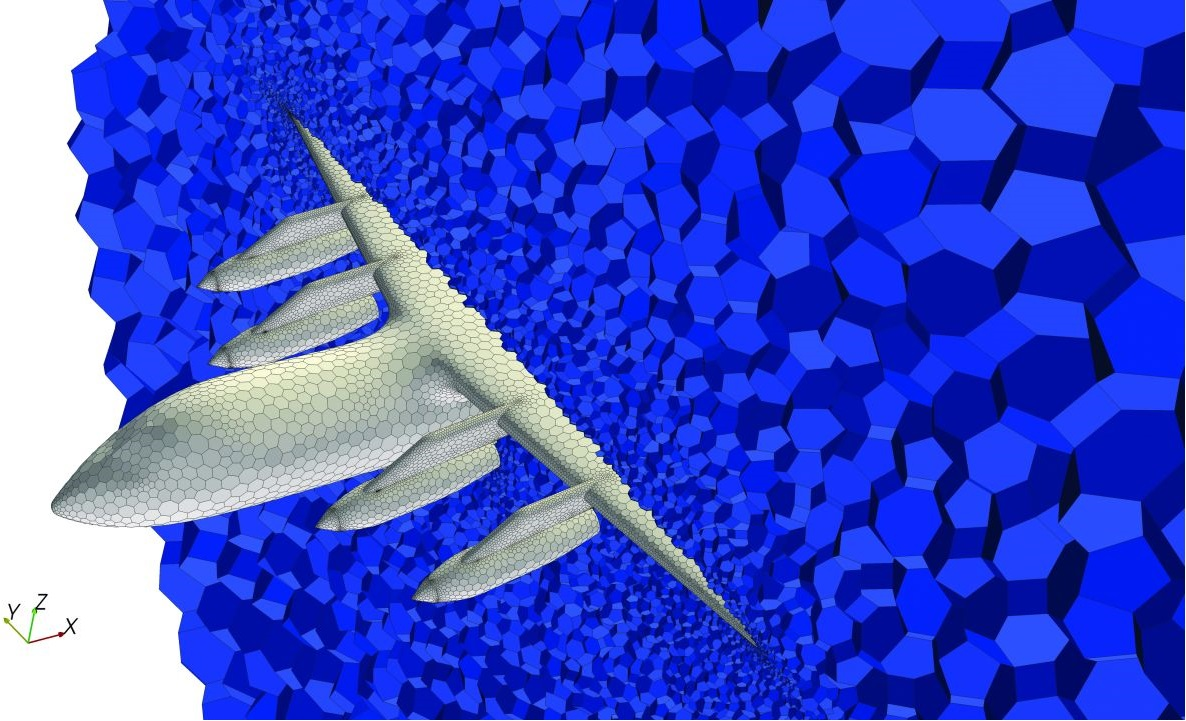
\includegraphics[width=0.45\columnwidth]{images/Polymesh_sized.jpg}
}
\only<2>{
{}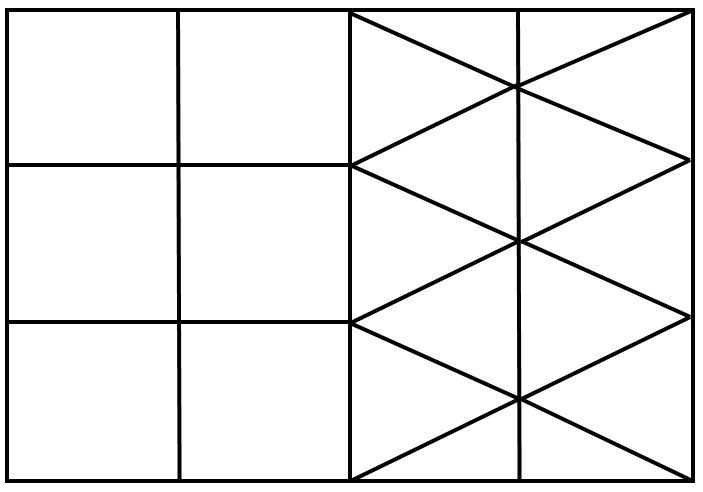
\includegraphics[width=0.4\columnwidth]{images/transition_elements.png}
}
\only<3>{
{}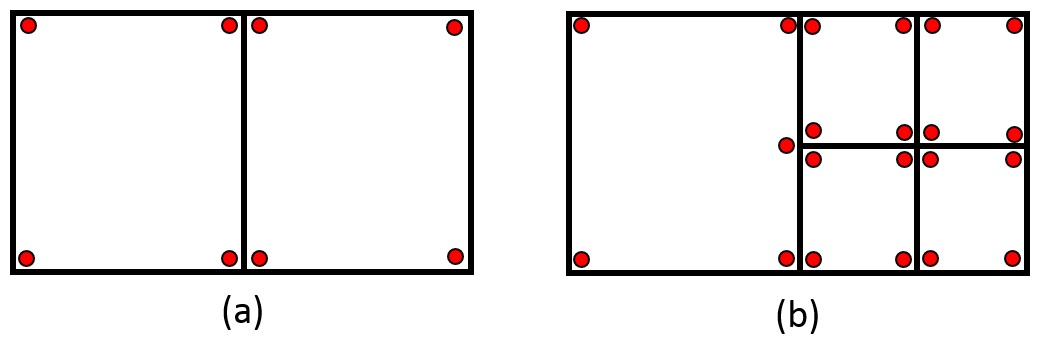
\includegraphics[width=0.55\columnwidth]{images/locally_refined_nodes.png}
}
\only<4>{
{}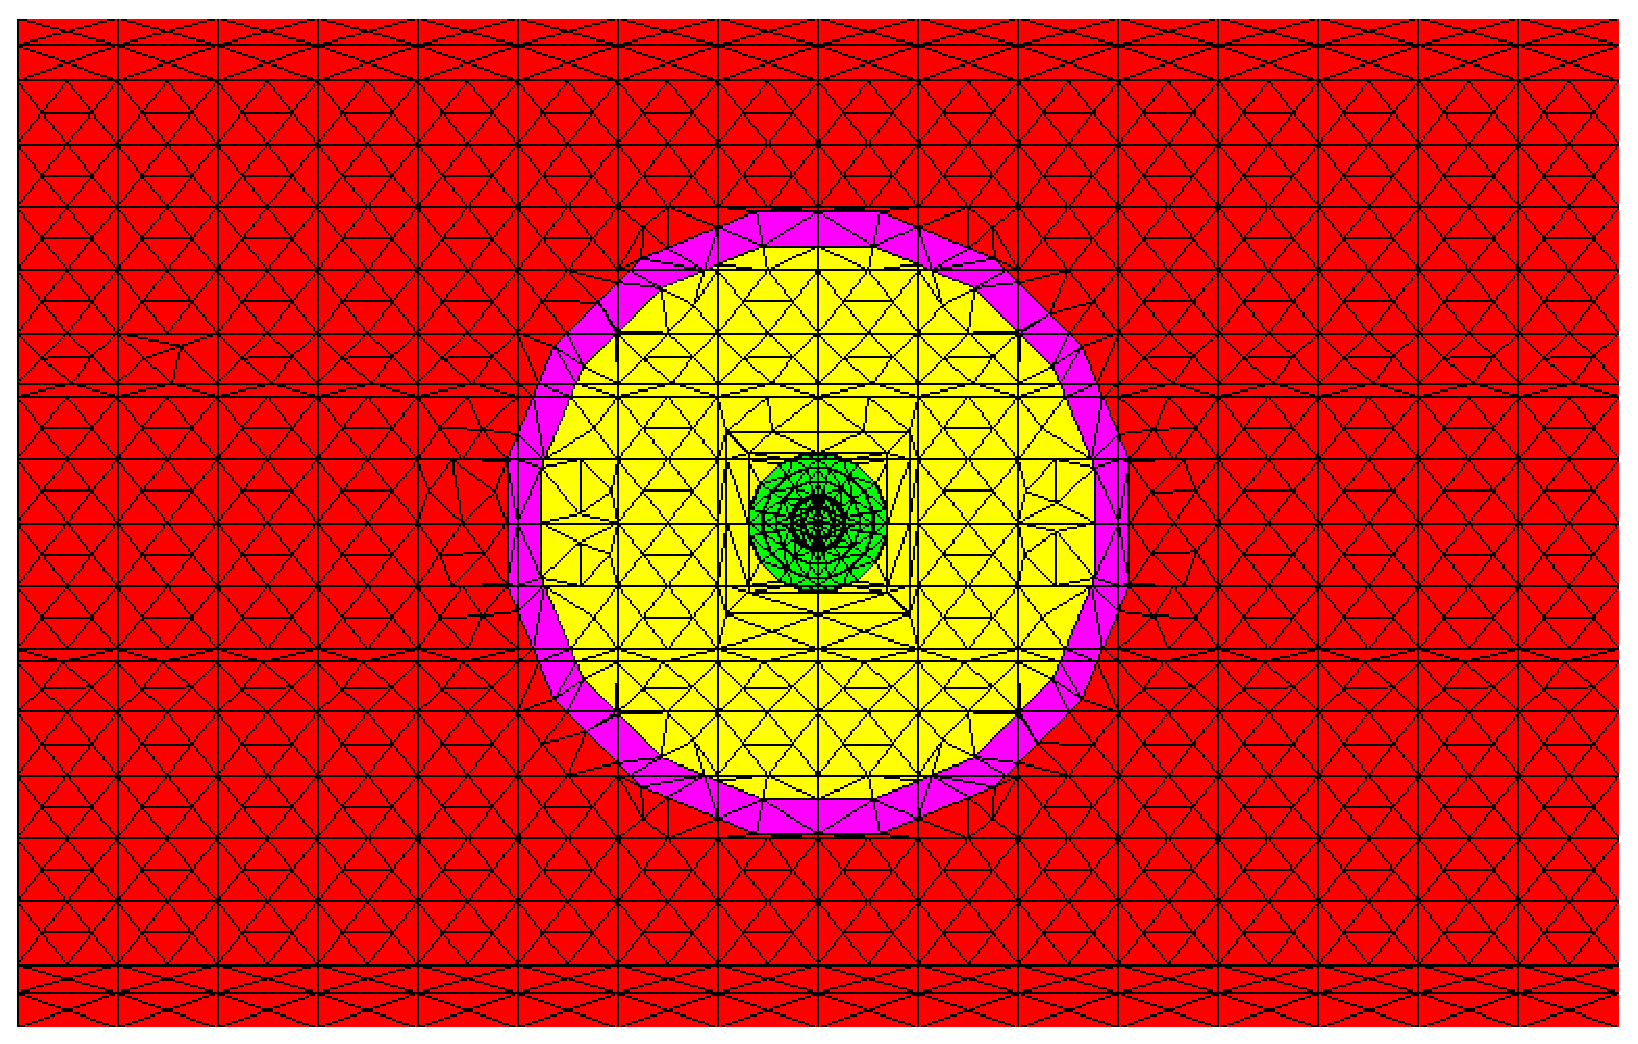
\includegraphics[width=0.50\columnwidth]{images/IM1_30_rot.eps}
}
\end{frame}
%%%%%%%%%%%%%%%%%%%%%%%%%%%%%%%%%%%%%%%%%%%%%%%%%%%%%%%%%%%%%%%%%%%%%%%%%%%%%%%%%%%%%%%%%%%%%%
%
%
\section[POLYFEM]{Polytope Finite Element Basis Functions}
%%%%%%%%%%%%%%%%%%%%%%%%%%%%%%%%%%%%%%%%%%%%%%%%%%
\subsection{Linear Basis Functions on 2D Polygons}
%%%%%%%%%%%%%%%%%%%%%%%%%%%%%%%%%%%%%%%%%%%%%%%%%%%%%%%%%%%%%%%%%%%%%%%%%%%%%%%%%%%%%%%%%%%%%
\typeout{***********************************************************************************}
\typeout{Linear Basis Functions on 2D Polygons}
%---------------------------
\setbeamerfont{frametitle}{size=\normalsize}
\begin{frame}\frametitle{Arbitrary Polygon and Definitions}
\centering
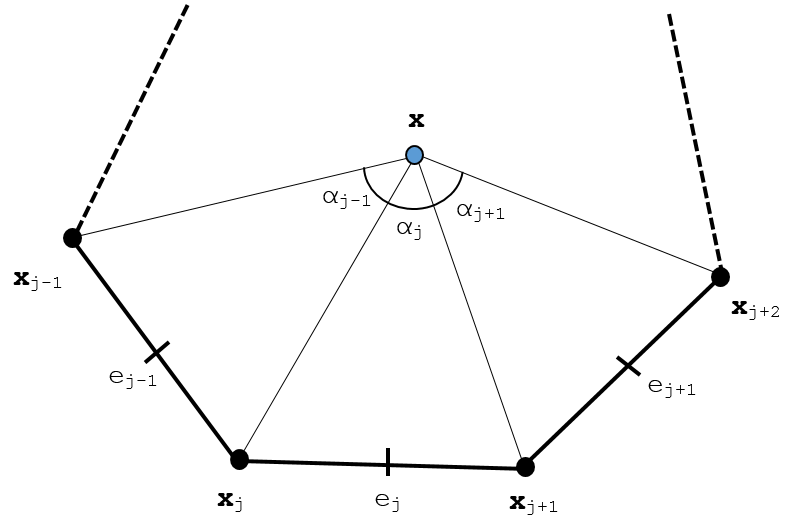
\includegraphics[width=0.50\textwidth]{images/ref_polygon.png}
\begin{block}{2D Linear Basis Function Properties - Barycentric Coordinates}
	\begin{enumerate}
	\item $\lambda_i \geq 0$
	\item $\sum_i \lambda_i = 1$
	\item $\sum_i \vec{x}_i \lambda_i (\vec{x}) = \vec{x}$
	\item $\lambda_i (\vec{x}_j) = \delta_{ij}$
	\end{enumerate}
\end{block}
\end{frame}
%---------------------------
\begin{frame}[t]\frametitle{Wachspress Rational Functions}

\end{frame}
%---------------------------
\begin{frame}[t]\frametitle{Piecewise Linear Functions}

\end{frame}
%---------------------------
\begin{frame}[t]\frametitle{Mean Value Coordinates}

\end{frame}
%---------------------------
\begin{frame}[t]\frametitle{Maximum Entropy Coordinates}

\end{frame}
%---------------------------
%%%%%%%%%%%%%%%%%%%%%%%%%%%%%%%%%%%%%%%%%%%%%%%%%%
\subsection{Quadratic Serendipity Basis Functions on 2D Polygons}
%%%%%%%%%%%%%%%%%%%%%%%%%%%%%%%%%%%%%%%%%%%%%%%%%%%%%%%%%%%%%%%%%%%%%%%%%%%%%%%%%%%%%%%%%%%%%
\typeout{***********************************************************************************}
%---------------------------
\begin{frame}[t]\frametitle{Quadratic Serendipity Basis Functions on 2D Polygons}

\end{frame}
%---------------------------
\begin{frame}[t]\frametitle{}

\end{frame}
%---------------------------
%%%%%%%%%%%%%%%%%%%%%%%%%%%%%%%%%%%%%%%%%%%%%%%%%%
\subsection{Linear Basis Functions on 3D Polyhedra}
%%%%%%%%%%%%%%%%%%%%%%%%%%%%%%%%%%%%%%%%%%%%%%%%%%%%%%%%%%%%%%%%%%%%%%%%%%%%%%%%%%%%%%%%%%%%%
\typeout{***********************************************************************************}
\typeout{Polytope Finite Element Basis Functions}

\setbeamerfont{frametitle}{size=\large}
\begin{frame}{Linear Basis Functions on 3D Polyhedra}

\end{frame}

%%%%%%%%%%%%%%%%%%%%%%%%%%%%%%%%%%%%%%%%%%%%%%%%%%%%%%%%%%%%%%%%%%%%%%%%%%%%%%%%%%%%%%%%%%%%%%
%
%
\section[DSA on Polytopes]{Diffusion Synthetic Acceleration on Polytopes}
\subsection{Theory}
%%%%%%%%%%%%%%%%%%%%%%%%%%%%%%%%%%%%%%%%%%%%%%%%%%%%%%%%%%%%%%%%%%%%%%%%%%%%%%%%%%%%%%%%%%%%%
\typeout{***********************************************************************************}
\typeout{DSA}
%---------------------------
\begin{frame}[t]\frametitle{}

\end{frame}
%---------------------------
\begin{frame}[t]\frametitle{}

\end{frame}
%---------------------------
\subsection{MIP Diffusion Form}
%%%%%%%%%%%%%%%%%%%%%%%%%%%%%%%%%%%%%%%%%%%%%%%%%%%%%%%%%%%%%%%%%%%%%%%%%%%%%%%%%%%%%%%%%%%%%
\typeout{***********************************************************************************}
\typeout{DSA}
%---------------------------
\begin{frame}[t]\frametitle{The Diffusion Equation and Boundary Conditions}
	\begin{block}{The Diffusion Equation} {\small 
     		\begin{align*}
 	 		{ \small -{\bf \nabla} \cdot D {\bf \nabla} \Phi ({\bf r}) + \sigma \Phi ({\bf r}) = q ({\bf r}), \qquad  {\bf r} \in \mathcal{D} }
        	\end{align*} }
        	\end{block}
        	\begin{block}{Boundary Conditions} {\small 
		\begin{align*}
 	 		{ \small \Phi ({\bf r})  = \Phi_0 ({\bf r}) , \qquad {\bf r} \in \partial \mathcal{D}^d } \\
 	 		{ \small -D \partial_n \Phi ({\bf r})  = J_0 ({\bf r}) , \qquad {\bf r} \in \partial \mathcal{D}^n } \\
 	 		{ \small \frac{1}{4} \Phi ({\bf r})  + \frac{1}{2}D \partial_n \Phi ({\bf r})  = J^{inc} ({\bf r}) ,  \qquad {\bf r} \in \partial \mathcal{D}^r}
        		\end{align*} }
    \end{block}
\end{frame}
%---------------------------
\begin{frame}[t]\frametitle{Symmetric Interior Penalty (SIP) Form}
	\begin{block}{Bilinear Form}{\small
		\begin{gather*}
			 a( \Phi, b)  = \Big<  D \vec{\nabla}  \Phi , \vec{\nabla} b  \Big>_{\mathcal{D}} + \Big<  \sigma   \Phi ,  b  \Big>_{\mathcal{D}}    \\
			+  \Big\{ \kappa_e^{SIP} [\![   \Phi ]\!] , [\![  b ]\!]\Big\}_{E_h^i} - \Big\{  [\![   \Phi ]\!] , \{\!\{  D \partial_n b \}\!\}\Big\}_{E_h^i} -\Big\{ \{\!\{  D \partial_n  \Phi \}\!\} , [\![ b ]\!]\Big\}_{E_h^i} \\
			+ \Big\{ \kappa_e^{SIP}   \Phi ,   b \Big\}_{\partial \mathcal{D}^d} - \Big\{   \Phi  ,  D \partial_n b \Big\}_{\partial \mathcal{D}^d} - \Big\{   D 				\partial_n  \Phi ,   b \Big\}_{\partial \mathcal{D}^d}  +  \frac{1}{2} \Big\{    \Phi ,   b \Big\}_{\partial \mathcal{D}^r}
        	\end{gather*} }
\end{block}
\begin{block}{Linear Form}{\small
		\begin{align*}
			\ell (b) = \Big<  q, b  \Big>_{\mathcal{D}}  - \Big\{   J_{0}, b  \Big\}_{\partial \mathcal{D}^n} +  2 \Big\{   J_{inc}, b  \Big\}_{\partial 				\mathcal{D}^r} \\ + \Big\{ \kappa_e^{SIP}   \Phi_0 ,   b \Big\}_{\partial \mathcal{D}^d} - \Big\{   \Phi_0  ,  D \partial_n b \Big\}_{\partial 					\mathcal{D}^d} 
        	\end{align*} }
    \end{block}
\end{frame}
%---------------------------
\begin{frame}[t]\frametitle{SIP Penalty Coefficient}
\begin{block}{}{
	\begin{equation*}
		\kappa_e^{SIP} \equiv 
		\begin{cases}
		\frac{C_B}{2} \left(  \frac{D^+}{h^+} + \frac{D^-}{h^-}  \right) & , e \in E_h^i \\
		C_B \frac{D^-}{h^-}  & , e \in \partial \mathcal{D}
		\end{cases}
	\end{equation*}}
	\begin{equation*}
		C_B = c p (p+1)
	\end{equation*}
\end{block}
\begin{block}{}
$c$ - user defined constant ($c \geq 1$) \\
$p$ - polynomial order of the finite element basis ($1,2,3,...$) \\
$D^{(+/-)}$ - diffusion coefficient defined on the positive/negative side of a face\\
$h^{(+/-)}$ - orthogonal projection defined on the positive/negative side of a face
\end{block}
\begin{block}{}
	\begin{equation*}
		u^{\pm} = \lim_{s \rightarrow 0^{\pm}} u ({\bf r} + s {\bf n})
	\end{equation*}
\end{block}
\end{frame}
%---------------------------
\begin{frame}[t]\frametitle{Modified Interior Penalty (MIP) Form}
	\begin{block}{Diffusion Form}{\footnotesize
		\begin{gather*}
			 \Big<  D \vec{\nabla}  \Phi , \vec{\nabla} b  \Big>_{\mathcal{D}} + \Big<  \sigma   \Phi ,  b  \Big>_{\mathcal{D}}    \\
			+  \Big\{ \kappa_e^{MIP} [\![   \Phi ]\!] , [\![  b ]\!]\Big\}_{E_h^i} - \Big\{  [\![   \Phi ]\!] , \{\!\{  D \partial_n b \}\!\}\Big\}_{E_h^i} -\Big\{ \{\!\{  D \partial_n  \Phi \}\!\} , [\![ b ]\!]\Big\}_{E_h^i} \\
			+ \Big\{ \kappa_e^{MIP}   \Phi ,   b \Big\}_{\partial \mathcal{D}^{vac}} -  \frac{1}{2} \Big\{   \Phi  ,  D \partial_n b \Big\}_{\partial \mathcal{D}^{vac}} -  \frac{1}{2} \Big\{   D 				\partial_n  \Phi ,   b \Big\}_{\partial \mathcal{D}^{vac}}  \\
 = \Big<  q, b  \Big>_{\mathcal{D}}  
        	\end{gather*} }
\end{block}
	\begin{block}{MIP Penalty Term}{\footnotesize
		\begin{align*}
			\kappa_e^{MIP} = \max(\frac{1}{4},  \kappa_e^{SIP})
		\end{align*} }
	\end{block}
\end{frame}
%---------------------------
%%%%%%%%%%%%%%%%%%%%%%%%%%%%%%%%%%%%%%%%%%%%%%%%%%%%%%%%%%%%%%%%%%%%%%%%%%%%%%%%%%%%%%%%%%%%%%
%
%
\section{Proposed Work and Current Status}
\subsection{}
\begin{frame}[t]\frametitle{}
% ---> Define proposed work
\end{frame}
\subsection{}
%---------------------------
\begin{frame}[t]\frametitle{}
% ---> linear transport solutions
\end{frame}
%---------------------------
\begin{frame}[t]\frametitle{}
% ---> MMS transport
\end{frame}
%---------------------------
\begin{frame}[t]\frametitle{}
% --->Searchlight problem introduction
\end{frame}
%---------------------------
\begin{frame}[t]\frametitle{}
% --->SL relative outlet error plots
\end{frame}
%---------------------------
\begin{frame}[t]\frametitle{}
% --->SL outgoing flux
\end{frame}
%---------------------------
\begin{frame}[t]\frametitle{}
% --->SL AMR plots with solutions
\end{frame}
%---------------------------
\subsection{}
%---------------------------
\setbeamerfont{frametitle}{size=\small}
\begin{frame}[t]\frametitle{SIP exactly linear solutions on 3D polyhedral meshes using the PWL basis functions}
\centering
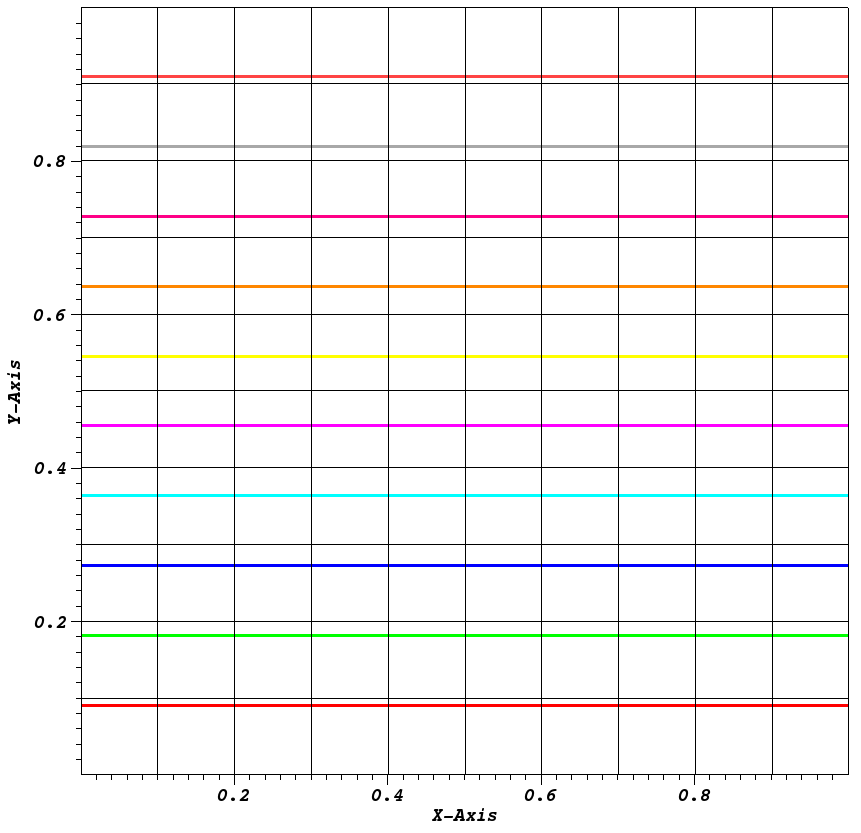
\includegraphics[width=0.32\textwidth]{images/cart_lin_contour.png} 
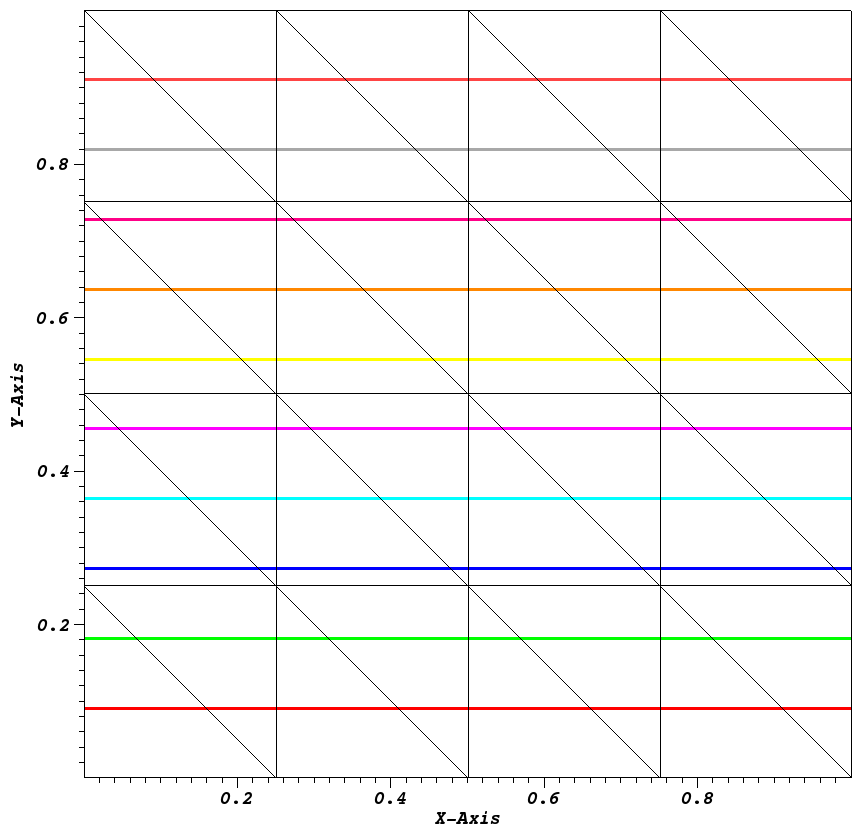
\includegraphics[width=0.32\textwidth]{images/tri_lin_contour.png} \\
\vspace{0.2cm}
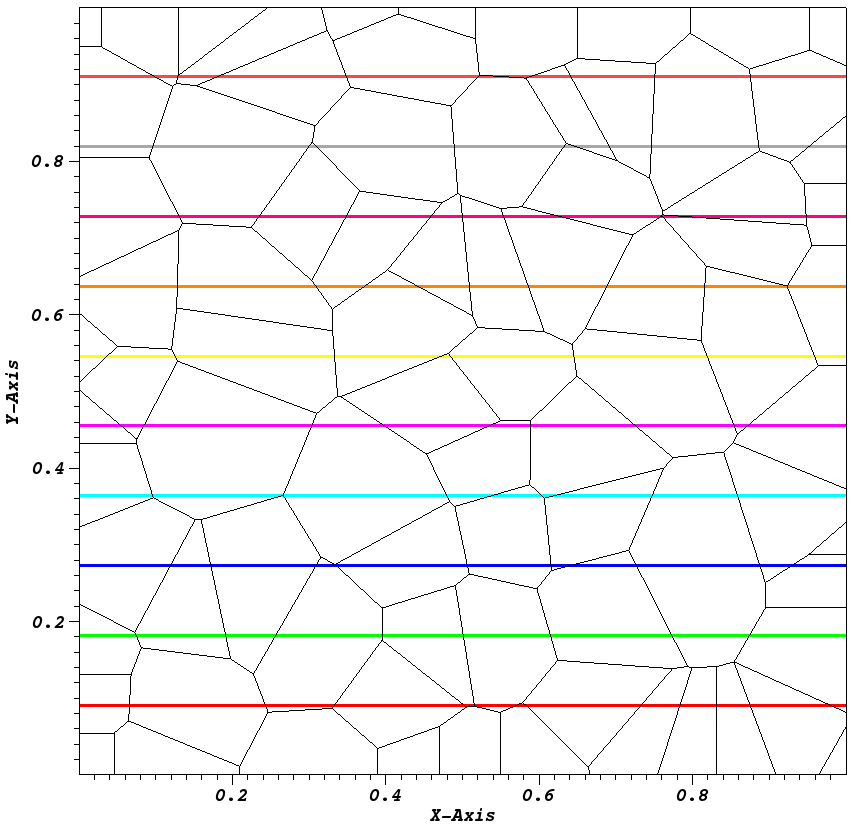
\includegraphics[width=0.32\textwidth]{images/poly_lin_contour.png} 
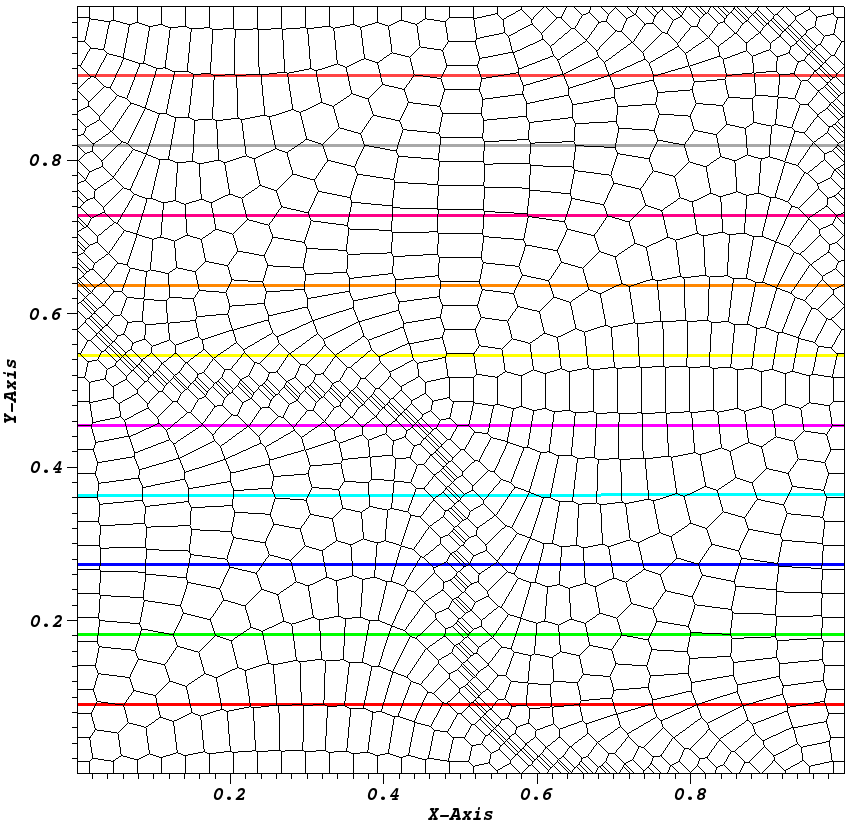
\includegraphics[width=0.32\textwidth]{images/sine_poly_lin_contour.png} 
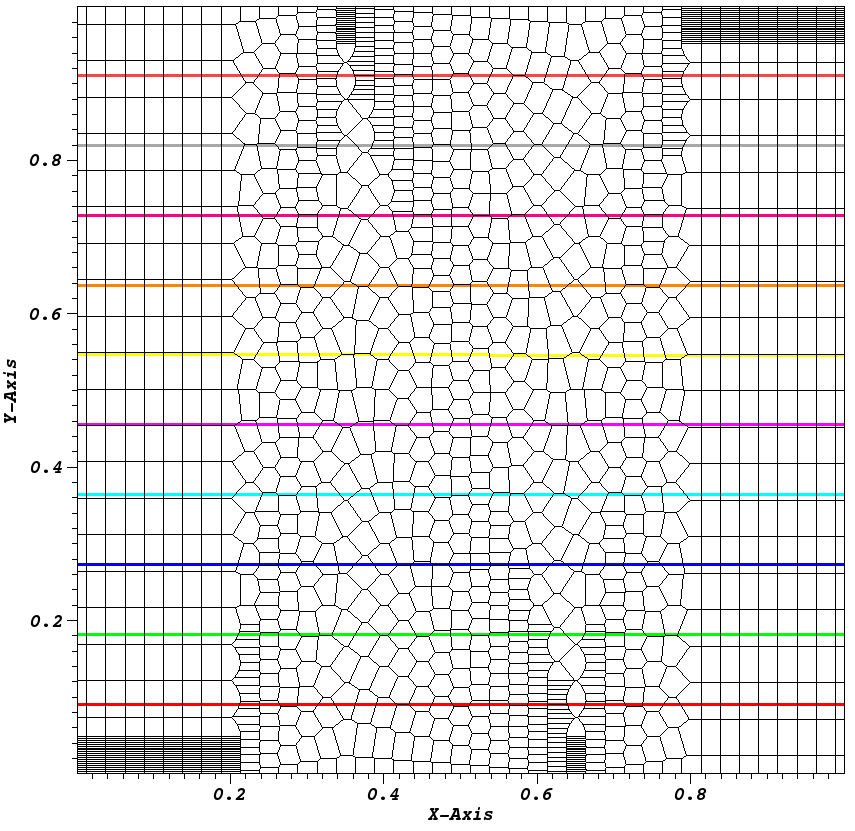
\includegraphics[width=0.32\textwidth]{images/z_poly_lin_contour.png} 
\end{frame}
%---------------------------
\setbeamerfont{frametitle}{size=\small}
\begin{frame}[t]\frametitle{SIP convergence study - quadratic solution on 3D cube using the PWL basis functions}
\begin{block}{}
	\begin{equation*}
		\begin{aligned}
		\Phi(x,y,z) =& x y z (L_x - x)  (L_y - y)  (L_z - z) \\
		L_x& = L_x = L_x = 1.0
		\end{aligned}
	\end{equation*}
\end{block}
\centering
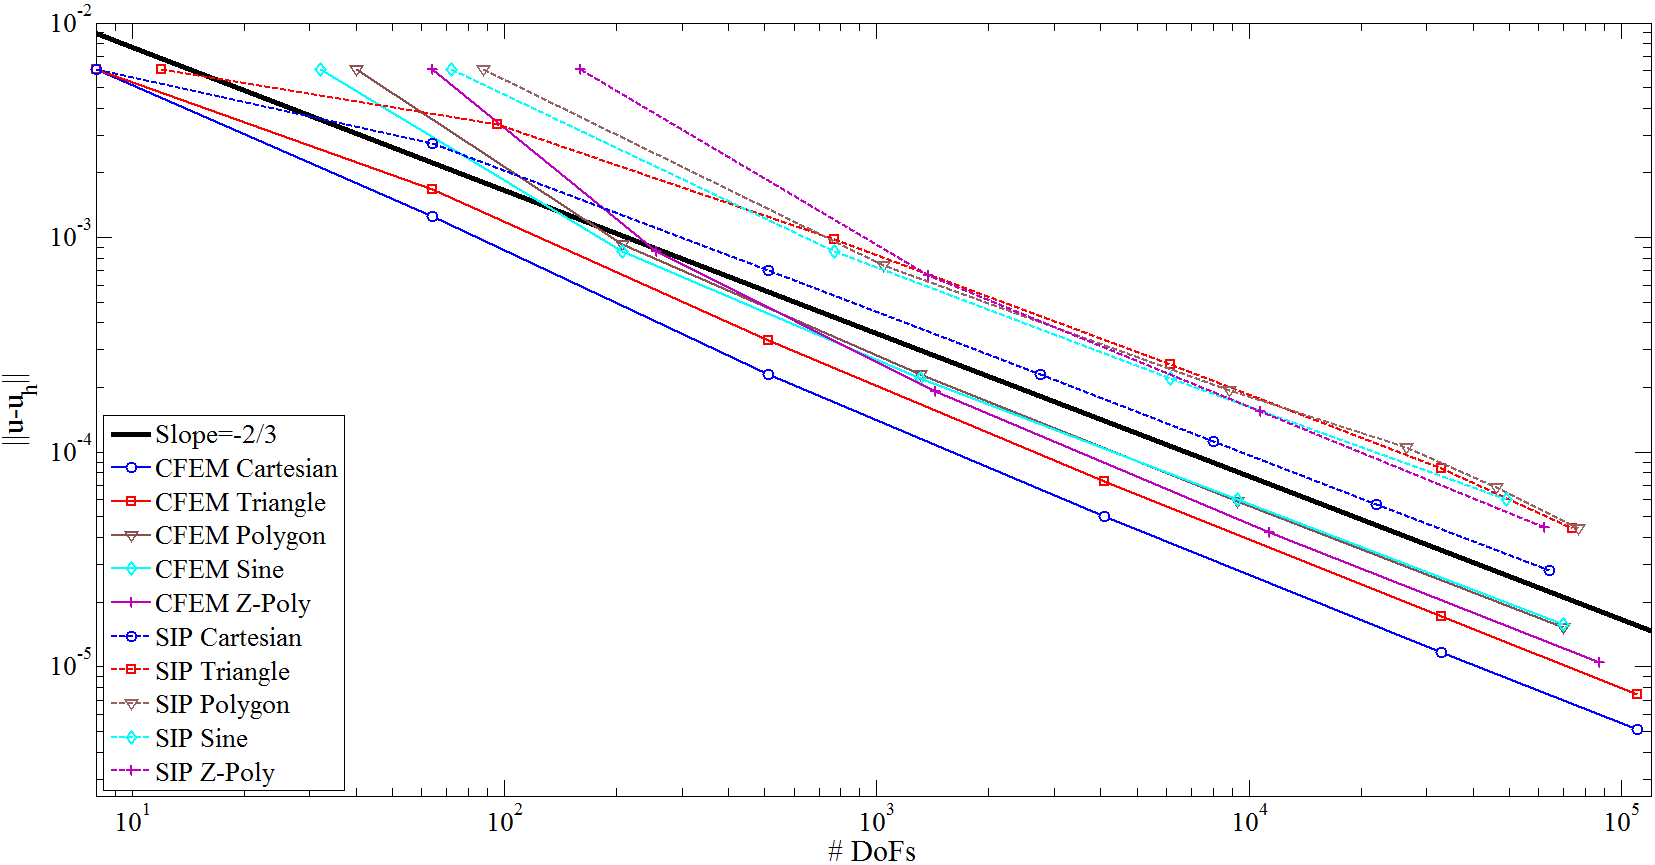
\includegraphics[width=0.9\textwidth]{images/sip_quad_full_paint.png} 
\end{frame}
%---------------------------
\setbeamerfont{frametitle}{size=\small}
\begin{frame}[t]\frametitle{SIP convergence study - gaussian solution on 3D cube using the PWL basis functions}
\begin{block}{}
	\begin{equation*}
		\begin{aligned}
		\Phi(x,y,z) = x y z (L_x - x)  (L_y - y)  (L_z - z) \exp(-({\bf r} - {\bf r}_0) \cdot ({\bf r} - {\bf r}_0))\\
		L_x = L_x = L_x = 1.0 , \qquad {\bf r}_0 = (3/4,3/4,3/4)
		\end{aligned}
	\end{equation*}
\end{block}
\centering
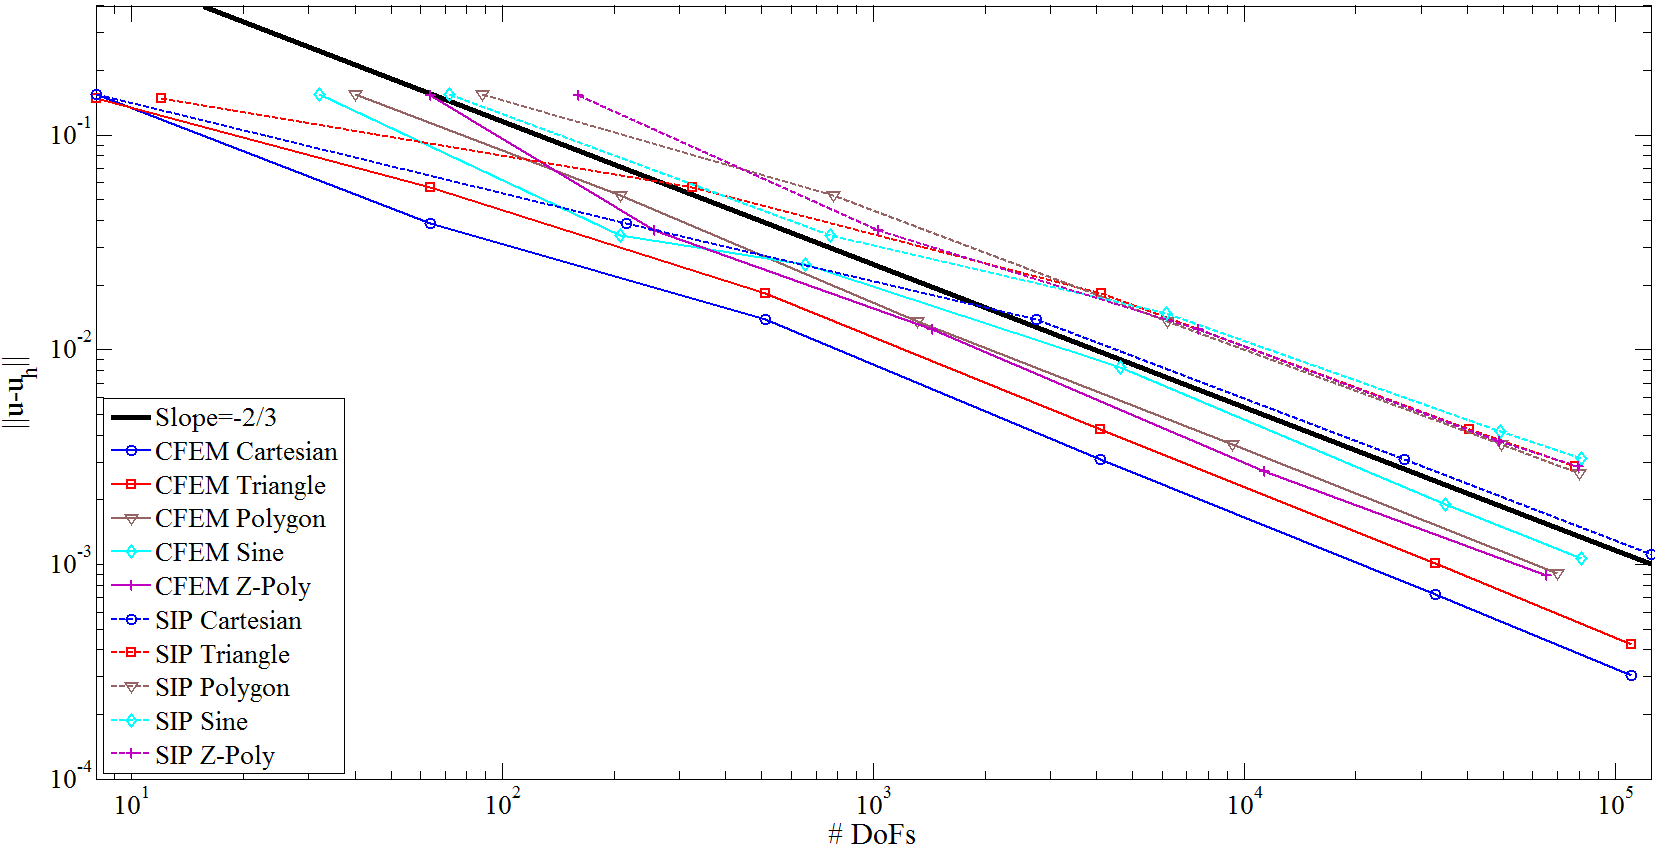
\includegraphics[width=0.9\textwidth]{images/sip_gauss_full_paint.png} 
\end{frame}
%---------------------------
\begin{frame}[t]\frametitle{}
% ---> 2D square fourier analysis
\end{frame}
%---------------------------
\begin{frame}[t]\frametitle{}
% ---> 2D aspect ratio fourier analysis
\end{frame}
%---------------------------
\begin{frame}[t]\frametitle{MIP DSA Timing Data with PDT on Vulcan using HYPRE}
\begin{figure}[t]
\centering
{}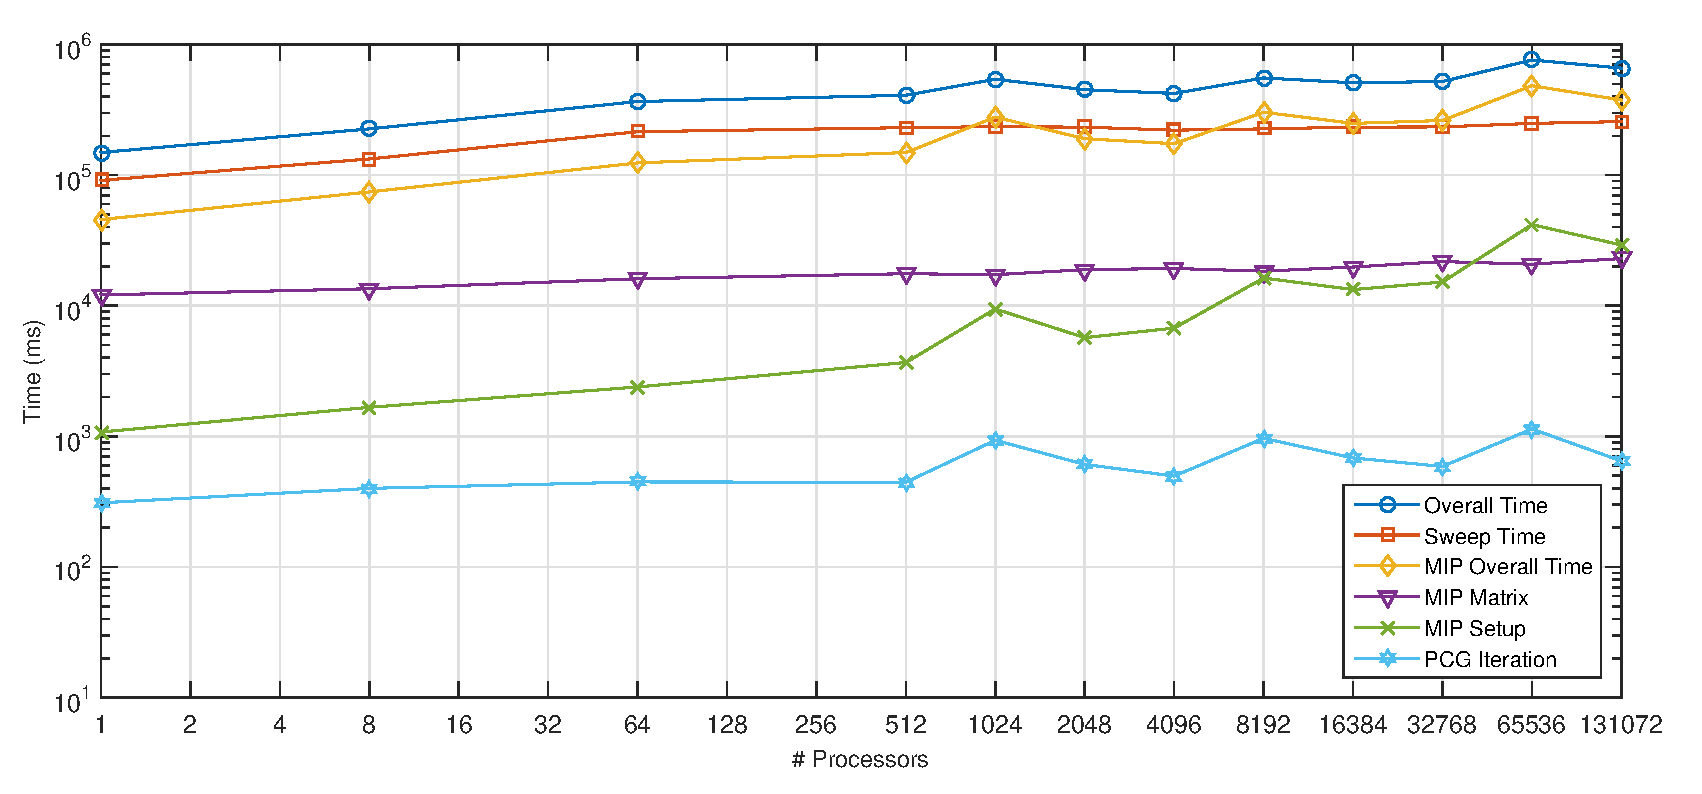
\includegraphics[width=0.75\textwidth]{images/Vulcan_DSA_Timing.eps}
\begin{block}{Problem Description}
	\begin{itemize}
	\item Modified Zerr problem - used optimal sweep aggregation parameters
	\begin{itemize}
	\item homogeneous cube - c=0.9999
	\item $S8$ level-symmetric quadrature
	\end{itemize}
	\item pointwise convergence tolerance of 1e-8
	\item precondition with MIP DSA using HYPRE PCG and AMG
	\end{itemize}
\end{block}
\end{figure}
\end{frame}
%---------------------------
\begin{frame}[t]\frametitle{}
% ---> Vulcan HYPRE parametric study results
\end{frame}
%---------------------------
%%%%%%%%%%%%%%%%%%%%%%%%%%%%%%%%%%%%%%%%%%%%%%%%%%%%%%%%%%%%%%%%%%%%%%%%%%%%%%%%%%%%%%%%%%%%%

\section{Ongoing Work}

%%%%%%%%%%%%%%%%%%%%%%%%%%%%%%%%%%%%%%%%%%%%%%%%%%%%%%%%%%%%%%%%%%%%%%%%%%%%%%%%%%%%%%%%%%%%

%\section{Conclusions}
% You need an empty subsection, or you don't get the little menu things.
%\subsection{}

%%%%%%%%%%%%%%%%%%%%%%%%%%%%%%%%%%%%%%%%%%%%%%%%%%%%%%%%%%%%%%%%%%%%%%%%%%%%%%%%%%%%%%%%%%%%%
\typeout{***********************************************************************************}
\typeout{We have reached the end}

\begin{frame}[plain]
   \frametitle{I look forward to your feedback regarding my PhD Proposal}

\vspace{25mm}

\begin{columns}[b]

\column{0.7\textwidth}

\centering

{\Large Questions?}

\vspace{9mm}
\footnotesize
A special acknowledgment to the Department of Energy Rickover Fellowship Program in Nuclear Engineering, which provides strong support to its fellows and their professional development.

\end{columns}

\vspace{10mm}

\begin{columns}[b]

\column{0.5\textwidth}
\centering
{}
\includegraphics[width=0.35\figwidth]{images/DOE_logo.png}\\

\column{0.5\textwidth}
\centering
{}
\includegraphics[width=0.70\figwidth]{images/tamu_engineering.png}\\

\end{columns}

\end{frame}

%%%%%%%%%%%%%%%%%%%%%%%%%%%%%%%%%%%%%%%%%%%%%%%%%%%%%%%%%%%%%%%%%%%%%%%%%%%%%%%%%%%%%%%%%%%

\backupbegin
\appendix

%%%%%%%%%%%%%%%%%%%%%%%%%%%%%%%%%%%%%%%%%%%%%%%%%%%%%%%%%%%%%%%%%%%%%%%%%%%%%%%%%%%%%%%%%%%%

\section{Backup Slides}

%%%%%%%%%%%%%%%%%%%%%%%%%%%%%%%%%%%%%%%%%%%%%%%%
\subsection{``Extra Credit''}

%%%%%%%%%%%%%%%%%%%%%%%%%%%%%%%%%%%%%%%%%%%%%%%%%%%%%%%%%%%%%%%%%%%%%%%%%%%%%%%%%%%%%%%%%%%%
\typeout{***********************************************************************************}
\typeout{Extra Credit Work}

\setbeamerfont{frametitle}{size=\large}
\begin{frame}
    \frametitle{A stretch goal is to compare my method to Monte Carlo}
    \framesubtitle{I claim the following is the best way to show our method has practical importance, because continuous-energy Monte Carlo codes do exact particle tracking / kinematics and use very accurate cross sections. Such codes may attain higher fidelity in all respects than DRAGON.}

    \onslide<1->{
    \begin{block}{Start with a 0-D problem to isolate energy discretization effects}
        \begin{enumerate}
            \item Come up with a reactor-themed problem
            \item Solve the same problem in PDT and MCNP or OpenMC
            \item Choose QOI, such as $k$-eigenvalue, radial power profile, absorption/fission rates per nuclide, etc.
            \item Quantify how errors in PDT's QOI change as energy resolution is increased
         \end{enumerate}
     \end{block}
     }
    \onslide<2->{
    \begin{block}{Build up problem complexity slowly: cylindricized pin cell with white boundary conditions, infinite lattice of pin cells, heterogeneous lattice of pin cells, etc.}
        \begin{enumerate}
            \item Quantify how errors in PDT's QOI change as spatial / angular / scattering moment resolution is increased
            \item Quantify how errors in PDT's QOI change as energy resolution is increased
            \item \ldots
            \item Profit
         \end{enumerate}
    \end{block}
    }

\end{frame}

\backupend

\end{document}

